\documentclass[]{report}
\renewcommand\thesection{\arabic{section}}%for page numbering in arabics
\usepackage{graphicx,tabularx}%for figures and tables
\usepackage[utf8]{inputenc} %allows special characters such as ä, ö, ỳ
\usepackage[english]{babel}  %set the language to English
\usepackage[margin=1.5in]{geometry} %change page margins 
\usepackage{sectsty}%section headers
\usepackage{algpseudocode}
\usepackage{float}
\usepackage{algorithm}
\allsectionsfont{\sffamily\large}
\subsectionfont{\sffamily\normalsize}
\linespread{1.2}% line distance
\usepackage{lipsum}% http://ctan.org/pkg/lipsum
\usepackage{caption}%use for captions on tables
%use this exact command. The style and bibliographystyle has to be authoryear (Havard). The sorting is nyt: name, year, title so that the bibliography is sorted alphabetically. firstinits=true shortens the names: Albert Einstein -> A. Einstein
\usepackage[backend=bibtex,style=authoryear,bibstyle=authoryear,sorting=nyt,firstinits=true]{biblatex}
\setlength\parindent{0pt}%include this so that your paragraphs don't indent automatically
\addbibresource{report.bib} %this attaches your bib-file, your bibliography (must be in the same folder)
\usepackage[compact]{titlesec}%include title formatting package
\setcounter{secnumdepth}{5}

% Title Page
\title{Relationship between Time Complexity and Number of Elements, within different Sorting Algorithms.}
\author{Mino Karadzhov and Kestutis Dikinis}
\date{December 10th 2021 \\Module: SEAR \\Venlo, Limburg, Netherlands}


\begin{document}

\maketitle

\begin{abstract}
Sorting  collections of information is one of common usages of computers nowadays. Sorting operations could take place in many of our daily interactions with information systems. There are several different techniques for conducting a sorting operation and choosing the proper one can reap huge savings and even make some problems possible to be solved in general[1]. \\

One of the metrics for measuring Algorithm Performance is the Time Complexity, which corresponds to the Time required for a given algorithm to fully complete it's task. In our case, this means fully sorting a collection.There is a number of factors that can affect the Time Complexity in both negative and positive way. The number of elements for sorting is one such factor, but what is the exact way that it affect the Time Complexity of a Sorting Algorithm? \\

This Paper describes an experiment, under the form of an Empirical analysis of four different Sorting Algorithms(SelectionSort, HeapSort, BubbleSort and Quicksort), that has a goal of studying the relationship between Time Complexity and the Number of elements for sorting. The results show an overall positive relationship between the two variables. However, the experimental results also show us that the exact ratio of growth is not the same for every Sorting technique.
\pagenumbering{roman}

\end{abstract}

\tableofcontents
\setcounter{page}{3}
\listoffigures %UNCOMMENT IF YOU HAVE FIGURES
%\listoftables %UNCOMMENT IF YOU HAVE TABLES
\pagebreak

\pagenumbering{arabic}	
	
\section{Introduction}
The Purpouse of this section is to introduce what is sorting algorithms and history of them, so there is general understanding about what is sorting algorithm. Introduce sorting algorithms used in research to get principle of working of different algorithms. And most importantly introduce the main research question. Also, this section will discuss problems, considerations and the hypothesis.
The main question of this research is: How does the time complexity of different sorting algorithms changes with increasing number of elements? It is important to learn about time complexity of sorting algorithms as this discipline gives us the potential to reap huge savings, even to the point of enabling us to do tasks that would otherwise be impossible. [1]

\subsection{Context and Background}
	In computer science, a sorting algorithm is an algorithm that takes elements of a list and puts them into an order - ascending or descending. The most popular values used are numerical and lexicographical order. It is important to have efficient sorting for optimising other algorithms, such as merge and search algorithms, as they require data to be in sorted list.
	Whenever there is a problem to be solved, there are many ways to approach it. Even though all those approaches end up with the same result, the time it takes for each approach can be vastly different. And the best example of that is sorting algorithms.  
		
		\subsection{Modern Usage, developments}
		
		Sorting algorithms are everywhere in day-to-day life in digital world. Everywhere starting from file browser in a computer - you can sort files on any parameters. Galleries in mobile phones - images sorted by date, contacts sorted alphabetically . Searching for a product in online store will have an option to sort products in many ways. 
		Commercial computing: government organisations, financial institutions, and commercial enterprises organise much of this information by sorting it. Whether the information is accounts to be sorted by name or number, transactions to be sorted by time or place, mail to be sorted by postal code or address, files to be sorted by name or date, or whatever, processing such data is sure to involve a sorting algorithm somewhere along the way. [2]
		Numerical computations: Scientific computing is often concerned with accuracy (how close are we to the true answer?). Accuracy is extremely important when we are performing millions of computations with estimated values such as the floating-point representation of real numbers that we commonly use on computers. Some numerical algorithms use priority queues and sorting to control accuracy in calculations.All in all, all any and every kind of list there is has been sorted in some way or another, as it is hard for a human to make use of unsorted data.[2]
		
\subsection{Sorting algorithm explanations}
		Bubblesort is a simple sorting algorithm that belongs to the family of comparison sorting. It works by repeatedly stepping through the list to be sorted, comparing two items at a time and swapping them if they are in the wrong order. Bubblesort has a worst-case complexity O(n 2 ) and in the best case O(n). Its memory complexity is O(1). [2]

		Heapsort is a comparison-based sorting algorithm, and is part of the Selection sort family. Although somewhat slower in practice on most machines than a good implementation of Quicksort, it has the advantage of a worst-case O(n log n) runtime.[2]

		Mergesort belongs to the family of comparison-based sorting. It has an average and worst-case performance of O(n log n). Unfortunately, Mergesort requires three times the memory of in-place algorithms such as Insertionsort. [2]

		Selection sort belongs to the family of in-place comparison sorting. It typically searches for the minimum value, exchanges it with the value in the first position and repeats the first two steps for the remaining list. On average Selection sort has a O(n 2 ) complexity that makes it inefficient on large lists. Selection sort typically outperforms Bubblesort but is generally outperformed by Insertionsort.[2]

		On the other side of the sorting algorithm spectrum there is BogoSort. It was designed as a joke about how not to design sorting algorithms. BogoSort takes and randomly swaps places all elements of the list and repeats it until the list is sorted. Complexity of BogoSort algorithm is O((n+1)!).

\subsection{Hypothesis, Problems and Considerations}
Derived from main research question, we can make a hypothesis that we are going to see a growth of the Time Complexity, towards Size of Collection.
		\subsubsection{Time Complexity and the importance of it.}
		Time complexity or more known as big O notation is a equation that describes how the runtime scales in respect to input variables. As time complexity describes the relationship between runtime and input variables it can b e said, that big O notation is used to have a rough approximation of how the program will react to being scaled and when it ism used to solve larger problems. [7]
		\subsubsection{Factors, operating on Time Complexity.}
		Determining the time complexity of an algorithm is important, and is done by few steps:
			-Breaking algorithm into individual operations.
			-Calculating big O for each calculation.
			-Adding up big O of each operation.
			-Removing the constants.
			-Finding the highest order term.
		After following these steps algorithms big O is found.
		
		There are few common cases of big O:
		O(1) - determining if number is odd or even.
		O(log n) - Finding an item in a sorted array using a binary search.
		O(n2) - Bubble sort or Insertion sort.
		O(n!) - Solving the traveling salesman problem using just brute-force search.
		\subsubsection{Different methods of approaching our Research question.}
		\clearpage
\section{Methodology}
In order to either confirm or reject our initial hypothesis, an empirical analysis of certain sorting algorithms was conducted. This chapter of the paper describes the process of conducting the experiment and creating the proper experimental environment. The subject group of sorting algorithms includes: QuickSort, BubbleSort, SelectionSort and HeapSort. The main goal of the analysis is to observe changes of the time complexity and memory usage, when the same algorithm is given the task to sort a collection of a certain size and type.
 Each observation of our experiment includes a task of sorting, performed by one of the sorting algorithms from our subject group, performed on a collection of certain size, containing either numerical or character type of elements.\\
In order to conduct the Empirical Analysis, a custom-made Java application was developed and used in the process. The main purpose  of which is to create a proper experimental environment , that is going to allow close observation of each algorithm from our subject group. \\
The overall goal is to gain an output, which allows data analysis on the behaviour of time complexity and memory used when the size and type, of the collections for sorting, change. 
	\subsection{Working Implementation of our Algorithms.}
	One requirement of the empirical analysis is a working implementation of the Sorting Algorithms, which are going to be used for the experiment. Due to this, the Java programming language was used to create working implementations of each one of the four members of our subject group. All of the concrete implementations of the algorithms implement a common interface, towards which the testing is being conducted.
	\subsection{Developing and using our experimental environment.}
	In order to serve the need of a proper experimental environment  for conducting the Analysis, Petko was developed. Petko is the name of the custom-made  algorithm analysis tool, that generates unsorted collections of a fixed size and uses sorters(Sorting Algorithms) to conduct the sorting operation. The latter is being closely monitored and both the time and memory, required for each sorting is being recorded in an output file.. \\
	Each Algorithm is used to perform 36 different observations in two separate stages. Each Observation requires the algorithm to sort an unsorted collection of a pre-defined size and type. The size of the unordered collection grows with each following observation. During the first stage of observation, each algorithm is being used for performing an operation of sorting on numerical collection with number of elements 2, whereas the last(18th) observation provides the Algorithm with an unsorted collection of 262144 elements. \\
	The second stage of the experiment, follows the same procedure as the first one. The main difference is the type of collections for sorting. During this stage, all of the unsorted collections are consisted of charecter type of elements.
	 The growth of Collection Size is Logarithmic with base 2. Respectively, this means that the first collection for sorting is with size 2$^{1}$, whereas the collection for the last observation has a size equal to 2$^{18}$. The values within the unsorted collections were numeral\\
	Petko actively uses the Java.time and Java.Runtime integrated libraries, in order to measure the Duration of time and memory used, between the start and end of the sorting process. \\
	Capturing the time complexity is made possible, by placing an Instant at the Start and End point of each Algorithm execution. The following PseudoCode provides a brief description of the technique:
	

\begin{algorithm}
	\caption{Capturing time complexity within Petko}\label{alg:cap}
	\begin{algorithmic}
	\State $startPoint \gets Instant.now()$   \Comment{Placing a start point, right before the start of a sorting operation}
	\State $sort()$
	\State $endPoint \gets Instant.now()$
	\State $timeComplexity \gets Duration.between(startPoint, endPoint)$
	\end{algorithmic}
\end{algorithm}

In order to get a record of the used memory, Petko is using 

	\newpage
		 Each Observation records the Sorting Algorithm that is being used, the TimeComplexity of the observation and the Size of Collection. This output is being gathered and recored into an external File under the .csv extension. 
		\subsection{Data Analysis and Visualisation}
		Petko's output file provides a great base for conducting Data Analysis on the results of the observations. By doing this, it is possible to identify and study certain patterns in the covariation between Time Complexity and Size of Collection. The same output file was imported into R and the findings were visualised, thanks to the tidyverse library.
		\section{Results}
	This section provides a detailed overview of the experimental results.
\subsection{Experimental Results}
After conducting the Emperical Analysis, 72 datapoints were generated. The same visualised on a ScatterPlot have the following view:

\begin{figure}
	\centering
	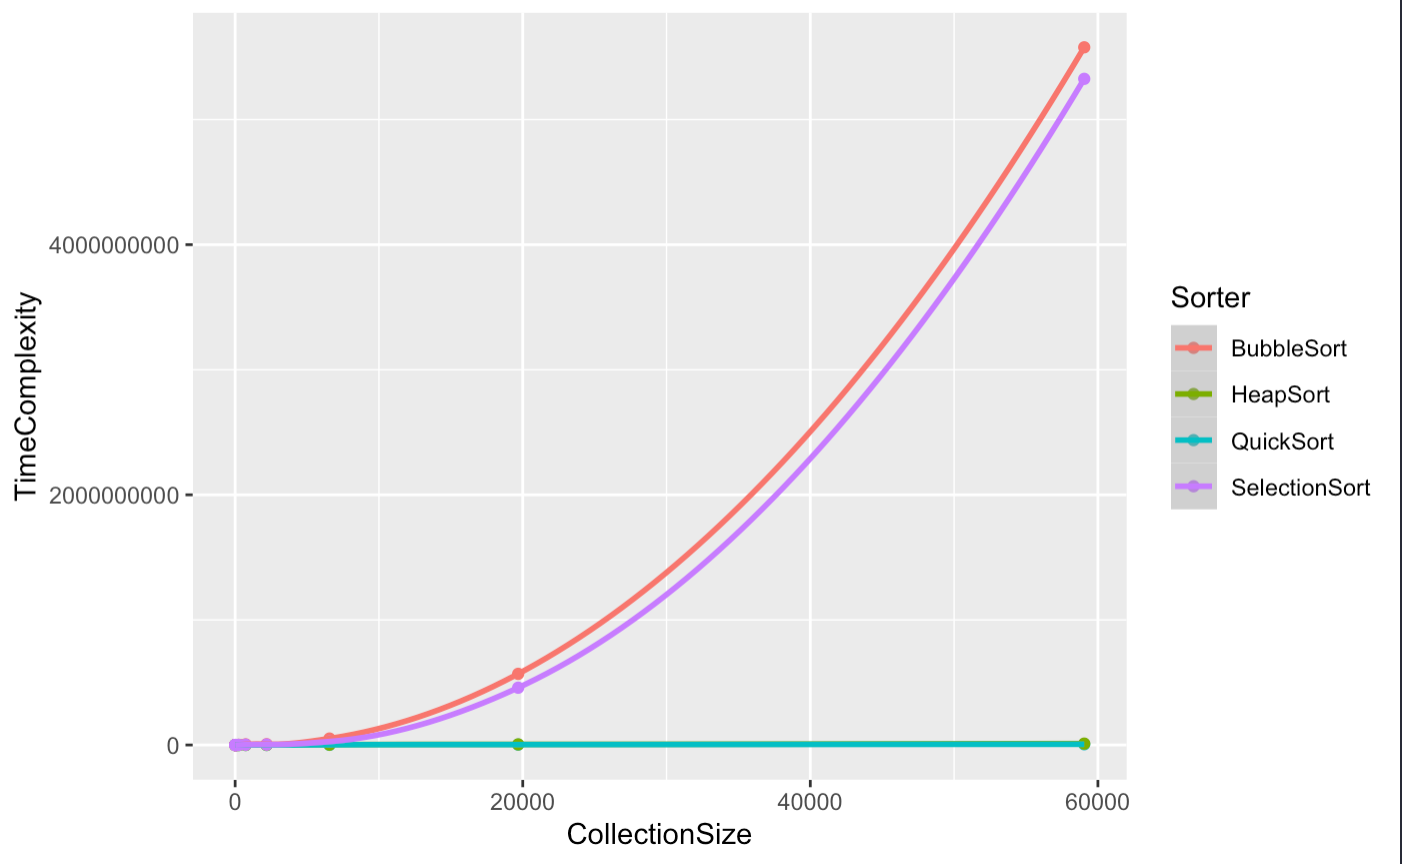
\includegraphics[width=0.7\linewidth]{ResultsOverallView}
	\caption[Figure 3.1:]{Overall view of the Experimental results.}
	\label{fig:resultsoverallview}
\end{figure}
\newpage
As we can clearly see from the above diagram, the relationship between Time Complexity and Collection Size differes between each one of the Sorters. In addition to this, we can easily identify a sharp growth of BubbleSort and SelectionSort time complexities, when the Collection size becomes more than 20 000 elements. On the other hand, looking at the QuickSort and HeapSort, we can easily observe a relationship, which can be described as similliar to Constant Time Complexity.
Taking the above into account, we can easily identify 2 sub-groups of sorters - One, where  TimeComplexity appears to be constant and One, where we can clearly see a Time Complexity growth, similliar to a Linear Growth.\\
Since the two sub-groups are vastly contrasting on the Overall view, this may be a reason why we are missing certain patterns on our visualisation.

\begin{figure}
	\centering
	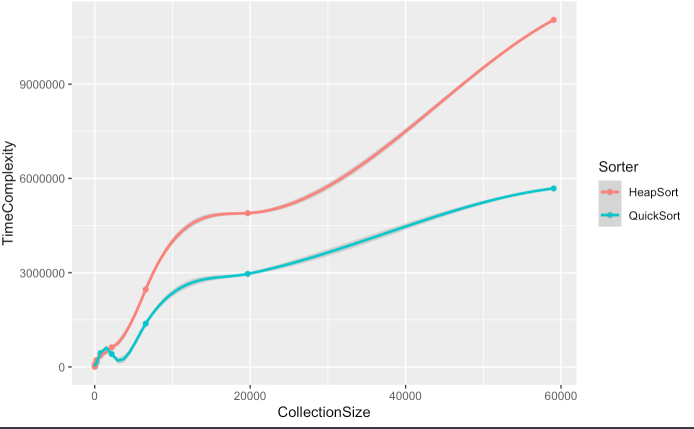
\includegraphics[width=0.7\linewidth]{OverviewOfConstantTimeComplexityAlgorithms}
	\caption[Figure 3.2]{Focused view on the sub-group with lower time complexity.}
	\label{fig:overviewofconstanttimecomplexityalgorithms}
\end{figure}
\newpage	
After creating a separate visualisation for the sub-group with lower Time Complexity, we can see more regarding the growth of Time Complexity, as the overlapping on the overal view did not provide a high level of detail. From the focuesed view, we clearly see that the Sorter with the lowest Time Complexity is the QuickSort, which is being followed by the other member of the sub-group - HeapSort. In addition to this, we can spot a rapid growth in the TImeComplexity, where the CollectionSize is between 0 and 10 000. The same growth appears to be substantially bigger in the observations, that include HeapSort.

\begin{figure}
	\centering
	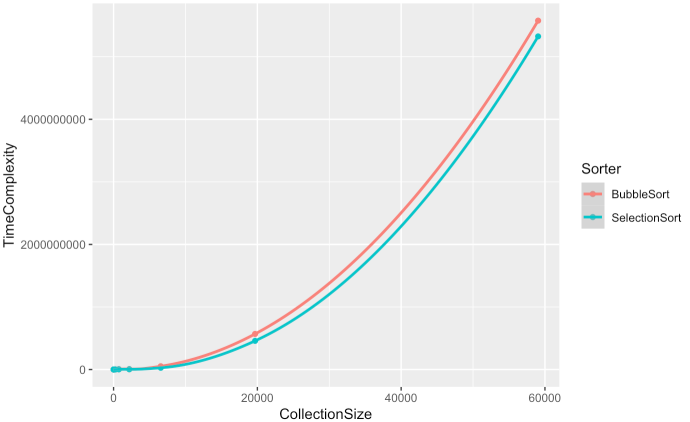
\includegraphics[width=0.7\linewidth]{FocusedViewOnBigTimeComplexity}
	\caption[Figure 3.3]{Focused view on the sub-group with higher time complexity}
	\label{fig:focusedviewonbigtimecomplexity}
\end{figure}
\newpage
Taking a focused look at the sub-group with higher time complexity, we can see that both of the sorters have a similar growth of Time Complexity, that leaves BubbleSort with slightly higher value of Complexity. The Growth here is similliar to a linear one and closer to the one that can be viewed on the Overall results view.
\section{Discussion}
In the following section we are going to discuss our results, give answer to our research question and provide a conclusion if our hypothesis was validated or not.
\subsection{Interpretation}
The Experimental results, clearly display a relationship, that can be described as a  positive correlation between Time Complexity and Collection Size. This validates our initial hypothesis, as the increased number of elements for sorting clearly results in an increase of the time required for completing the sorting operation. In addition to this, we gained knowledge, that shows that different Sorting techniques (Algorithms) are not being affected in the same way by the increased number of elements for sorting. For instance, on the Overall view of our Experimental results, we can see that BubbleSort and SelectionSort are experiencing a drastic increase of their TimeComplexity, whereas the other two Sorters - QuickSort and HeapSort are not following the same pattern.\\
Based on this, we can conclude that the latter group of Sorters can be a better choice for executing sorting tasks, which are placing their focus on the Time Resource being spend.
\subsection{Considerations}
This subsection describes the Considerations made during the Experiment, as well as reasoning for some of the decisions described in the Methodology section.
\subsubsection{Limitations of the Empirical type of Analysis}
It has to be taken into account that the Empirical way of conducting the Analysis is not the best, in terms of time efficiency. That is due to the fact that this type of analysis, requires a working implementation of the subjects(Sorting Algorithms) that are going to be analysed. \\
Furthermore, a certain amount of computing power is required, as this type of analysis requires the Algorithms to be put into action. In order to experiment with bigger Collections, which could be beneficial for revealing (otherwise hidden) patterns, larger amount of computing power is going to be required. 

\subsubsection{Limitations of the Collection Size}
Because of the nature of Empirical Analysis, described in the last sub section, this experiment used Collections of size, just up to 2$^{18}$ - 262144 elements.This limitation was present, mainly due to the fact that the machine, we used for testing, was not capable of experimenting with bigger collections. Would we have more computing power at our disposal, there could've been more patterns and datapoints to extend the scope of the experiment.
\subsubsection{Limitations of the Machine, used for the Experiment}
The described experiment was conducted on a Machine with the following technical specifications : CPU: 2 GHz Quad-Core Intel Core i5, 16 GB 3733 MHz LPDDR4X RAM. In addition to the Collection Size limitation, it is worth considering the fact that our experimental results were somehow influeced by the computational power, available with the above specifications. This means, that there is a high chance of observing different time complexity values, if the same experiment is conducted on another machine.
\subsection{Evaluations}
	As this experiment is being conducted in a relatively small scope, taking into account the limited size of collections used, there could be an argument that this limits us from seeing how the Relationship between Time Complexity and Size of Collection changes with having bigger collections for sorting. This argument can be taken as a valid one, as the described experiment does not take into account Collections of much larger size. \\
	
	Taking this argument into account, we can evaluate that this study can serve as the base idea of conducting further experiments, that will provide insights based on a larger scope of Collection sizes. The same will make possible to study the patterns and changes in the relationship of Time Complexity and number of elements for sorting, within bigger collections.
 \end{document}
	
	
\printbibliography[title=References]
R. Lafore. Data Structures and Algorithms in Java. SAMS
Publishing, Indianapolis, Indiana, USA, 2nd edition, 2002.

[2]Bunse, C., Hopfner, H., Mansour, E. and Roychoudhury, S., n.d. Exploring the Energy Consumption of Data Sorting Algorithms in Embedded and Mobile Environments. [online] citeseerx.ist.psu.edu. Available at: <https://citeseerx.ist.psu.edu/viewdoc/download?doi=10.1.1.543.8109&rep=rep1&type=pdf> [Accessed 14 December 2021].

[1]Sedgewick, R. & Wayne, K. (2011), Algorithms, 4th Edition. , Addison-Wesley .

[4]R. Sedgewick, Algorithms in C++, Addison–Wesley Longman,1998,pp 273–274.

[5]A.  Levitin, Introduction to the Design & Analysis of Algorithms,  Addison–Wesley Longman, 2007, pp 98–100.

[6]https://en.wikipedia.org/wiki/Sorting_algorithm

[7]Mohr, Austin. "Quantum Computing in Complexity Theory and Theory of Computation" (PDF). p. 2. Retrieved 7 June 2014.
\end{document}
